\documentclass{mefsdp}


\setauthors{Alp Gokcek, Erdal Sidal Dogan}
\settitle{TURKISH QUESTION GENERATION MODEL}
\setcourseno{II}
\setmonth{June}
\setyear{2021}
\setfaculty{Engineering}
\setdepartment{Computer Engineering}
\setchair{Prof. Muhittin Gokmen}
\setdate{05/06/2021}
\setadvisor{Asst. Prof. Seniz Demir}

\settitleTR{TÜRKÇE SORU OLUŞTURMA MODELİ}
\setmonthTR{Haziran}
\setfacultyTR{Mühendislik}
\setdepartmentTR{Bilgisayar Mühendisliği}
\setadvisorTR{Dr. Şeniz Demir}

\setfigurepath{../figures/}


\newacronym{dl}{DL}{Deep Learning}
\newacronym{qg}{QG}{Question Generation}
\newacronym{nlp}{NLP}{Natural Language Processing}
\newacronym{do}{DÖ}{Derin Öğrenme}
\newacronym{su}{SÜ}{Soru Üretme}
\newacronym{ddi}{DDİ}{Doğal Dil İşleme}

\usepackage{xcolor}
\usepackage{natbib}
\usepackage{fancyvrb}
\usepackage{fvextra}

% redefine \VerbatimInput
\RecustomVerbatimCommand{\VerbatimInput}{VerbatimInput}%
{fontsize=\footnotesize,
	%
	frame=lines,  % top and bottom rule only
	framesep=2em, % separation between frame and text
	rulecolor=\color{black},
	%
	labelposition=topline,
	%
	commandchars=\|\(\), % escape character and argument delimiters for
	% commands within the verbatim
	commentchar=*        % comment character
}

\begin{document}
	
	\makestandards
	
	\begin{abstract}
		Question Generation is a Deep Learning model that given a paragraph, passage or an entity in Turkish, produces the possible questions that can be answered solely by the given content to the system. \gls{qg} Systems are capable of generating various logical questions from the given text input. \gls{qg} Systems are prevalent in several computer applications such as chatbots, automated grading systems etc. \newline \par 
		
		In this project, our aim is to train a \gls{dl} model for question generation and assess its performance according to evaluation metrics. We find this task worth tackling since there are not many examples of comprehensive studies on the topic and the outcomes of this project will empower the development of more capable-than-ever Question Answering Systems for the Turkish Language.
		\gls{qg} models require extensively large training data, thus, in the last semester we have developed the initial dataset for the development of the \gls{qg} model. This dataset is the largest Turkish Question-Answer dataset currently available. In this project, our aim is to develop the first question generation model for Turkish language and assess its performance as well as improving the diversity of our dataset TurQuAd.

		\keywords{Artificial Intelligence, Natural Language Processing, Deep Learning, Question Generation}
	\end{abstract}
	
		
	\begin{abstractTR}
	\gls{su} Modeli, Türkçe bir paragraf, pasaj veya varlıktan, sadece verilen içerikle cevaplanabilecek olası soruları sisteme üreten bir \gls{do} modelidir. \gls{su} Sistemler, verilen metin girdisinden çeşitli mantıksal sorular üretebilir. \gls{su} Sistemler, sohbet robotları, otomatik derecelendirme sistemleri vb. gibi çeşitli bilgisayar uygulamalarında yaygındır. \newline \par
	
	Bu projede amacımız, soru oluşturma için bir \gls{do} modelleri eğitmek ve performansını değerlendirmektir. Konuyla ilgili çok fazla kapsamlı çalışma örneği bulunmadığından ve bu projenin çıktıları Türk Dili için her zamankinden daha yetenekli Soru Cevaplama Sistemlerinin geliştirilmesini güçlendireceğinden, bu görevi çözmeye değer buluyoruz.
	\newline \par 
	\gls{su} modelleri çok büyük eğitim verileri gerektirir, bu nedenle son dönemde \gls{su} modelinin geliştirilmesi için ilk veri kümesini geliştirdik. Bu veri kümesi, şu anda mevcut olan en büyük Türkçe Soru-Cevap veri kümesidir. Bu projede amacımız, soruların oluşturulması ve performanslarının değerlendirilmesi ve veri setimizin çeşitliliğinin iyileştirilmesi için bir derin öğrenme tabanlı bir soru üretme modeli yaratmaktır.
			
		\anahtarkelimeler{Yapay Zeka, Doğal Dil İşleme, Derin Öğrenme, Soru Üretme}
	\end{abstractTR}
	
	\makelists
	
	\section{Introduction}
	Artificial Intelligence is one of the promising research fields in computer science. Scientists and researchers are developing novel or more efficient ways to teach computers how to achieve humanly-kinds of tasks.\\
	
	Over time, developments in this area yield to a whole new class of possibilities and problems requiring brand new methodologies to reach the solution. With the emergence of Machine Learning, computers became to be able to parse data, learn from the data and apply their findings from it in a way that they are told to.\\
	
	In recent years, researchers came up with a more niche way of handling Machine Learning (ML) tasks, creating a structure that imitates the Neurons in our brains. This new subclass of ML is named Deep Learning (DL). Compared to ML, it is capable of handling a much more complicated task due to its multi-layered structure.\\
	
	Developments in this area enabled researches from numerous fields to move their research a step further. Today, Deep Learning is ubiquitous in computer applications. It is utilized for Computer Vision, Natural Language Processing, Biotechnology and much more. In this project, methods and techniques that are results of the studies conducted in the research area of Natural Language Processing are used heavily along with various Machine Learning and Deep Learning models. Consequently, the Turkish Question Generation is invigorated by the state-of-art Deep Learning and Language Models.\\
	
	Turkish Question Generation Model aims to generate natural language questions from a given content, such as paragraphs, where the questions can be answered solely by the content.   As the authors, we find this task worth tackling since there are not many examples of comprehensive studies on the topic and the outcomes of this project will empower the development of more-capable-than-ever Question Answering Systems for the Turkish Language. 
	\newpage
	
	\subsection{Motivation}
	
	As humans, we are continually learning, adapting to changes or make decisions on an everyday basis. Even if we do not realize, we usually are dependent on other humans and their knowledge and expertise even for most trivial things we do in our daily lives.\\
	
	For instance, a student feels in need for an instructor or others than can address his/her questions about a topic, an individual may be in a hurry to find out whether he/she can perform SWIFT transaction from his bank, or simply a person can ask about the weather forecast to the voice assistant on a smartphone. All of these examples are having a common point that they are all based on Question Answering (QA) Systems.\\
	
	As we have discussed, QA Systems are getting more and more space in our lives and presents a wide range of opportunities. With these systems, we are able to get answers to our question at no time, without any human interaction at all. This feature enables humans to reach to even the most isolated information in the context a matter of time upon request.\\
	
	Unfortunately, given that almost every human spoken language has a specific set of rules, grammar and vocabulary, QA systems need to be developed for each language separately. Development of such systems are not the easiest thing to do, first of all, even if the developer(s) has all the competency in the technical skills required, there is a need for clear, labelled, reliable and excessively large dataset. The dataset must contain questions and possible answers to that question. Creating such dataset manually is almost unattainable; therefore, there is a need for a system that can automate this process. Question Generation systems are perfect for meeting such need. The output of the QG system can be used as the dataset for development.\\
	
	On top of that, QG systems can be utilized in the education field also. Given a passage, the instructor may want to create various questions automatically without putting any effort. The same application can be used by a student for practising the learnings from a section.
	
	
	\subsection{Broad impact}
	\subsubsection{Global Impact of the solution}
	Online courses are gaining getting more and more popular each and every year. While their high-quality content is available on the web, for those who cannot understand English or mainstream languages of a specific subject, it is harder to keep up with the recent developments in the area. Up to this point, MOOC platforms offer translation and subtitles for such users. The Question Generation systems, along with Question Answering systems, might create an artificial interactive environment between the instructor and the student. Consequently, helping the information to spread around the world.
	
	\subsubsection{Economic Impact of the solution}
	This project enables us to move faster to the point where we can automate almost every Question-Answer process where the data is assumed to be available to a computer system; there is not an ambiguity amongst possible answers, and the answers are static and clearly defined or quantitative.\\
	
	Initial assumption would be that such a system would decrease human dependency and reduce the number of jobs consequently. However, given that the same approach is applicable to almost every new technology/product emerges in the market, it is shown that they also create new opportunities. 
	
	
	\subsubsection{Environmental Impact of the solution}
	Since the project will be software-based, no significant effect on the environment will be observed. Of course, one can discuss keeping the servers on, utilizing their resources to the maximum level continually will increase the total electricity consumption. 
	
	\subsubsection{Social Impacts of the solution}
	This project has many social impacts, though not directly. With the solution we developed, strengthening the question-answering model carried out in connection with this project, we will aid the learners' knowledge acquisition process.
	
	
	\subsubsection{Legal Issues related to the project}
	Such as any system that is designed to present information to the user, Question Answering systems, which our project Question Generation system will yield to development of, requires the necessary information for answering the question. Under these circumstances, the source of this information is critically important. Consent of the creator must be obtained before developing such a system. \\
	
	The system must also not give inaccurate information to the user, since they may depend on the system on a critical task whose fault cannot be tolerated.
	
	\section{Project Definition and Planning}
	Turkish Question Generation Model is a neural network-based model capable of generating questions from a given piece of text in the Turkish language.
	
	\subsection{Project Definition}
	The project's main feature will be accepting input and creating possible questions from that input while assigning probability scores to each generated question. Questions are delivered in easily parsable file format such as JSON, CSV etc.\\
	
	A GUI\footnote{Graphical User Interface} will be designed to demonstrate the capabilities and enable majority of people to use it without any technical knowledge. Also, it will be presented as CLI\footnote{Command Line Interface} and \textit{Python Module}\footnotemark \footnotetext{An importable Python file that contains the functions for incorporating Turkish Question Generation for further research.} servers for public use, if allowed.
	\\
	
	\begin{figure}[ht!]
		\centering
		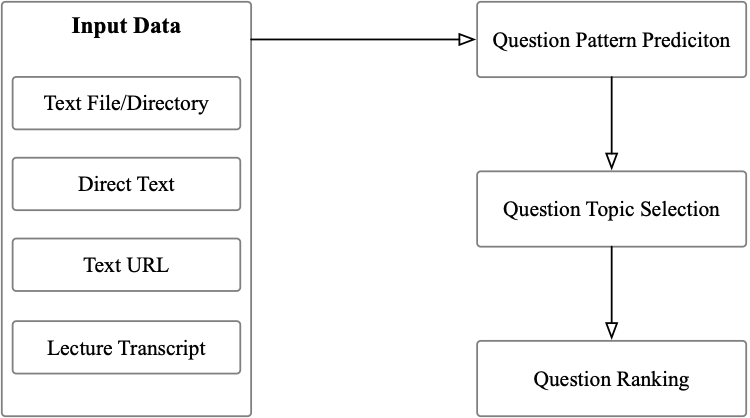
\includegraphics[scale=.8]{qg-system-schema}
		\caption{Question Generation system schema}
	\end{figure}
	
	\subsubsection{Dataset}
	There are lots of publicly available datasets for natural language processing tasks. However, for this project, our primary constraint was to build our system on top of a Turkish Dataset. Some other constraints we had was that the data must consist of correctly structured sentences in grammatical aspect, it must be labeled, come from a reliable source with the consent of the owner(s) and must be very large, given that larger dataset yields better models.
	
	\subsubsection{Programming Languages and Frameworks}
	This project is developed with \textit{Python 3}. It has chosen because it is relatively simple and allows us to focus on the project rather than computational concerns, it has a vast community for troubleshooting, decreasing the chances of having an issue about the language.\\
	
	Furthermore, Python is adapted by the AI researchers, and there are numerous resources, frameworks and libraries that are developed for Python in which we utilize heavily. We have not limited ourselves to a specific framework or library for the development of the models. Also, there are other libraries that are developed for scientific computing and have been used in this project such as \textit{pandas, NumPy}, etc.\\
	
	\subsection{Project Planning}
	\begin{table}[ht!]
		\caption{Project plan for 14 weeks}
		\centering
		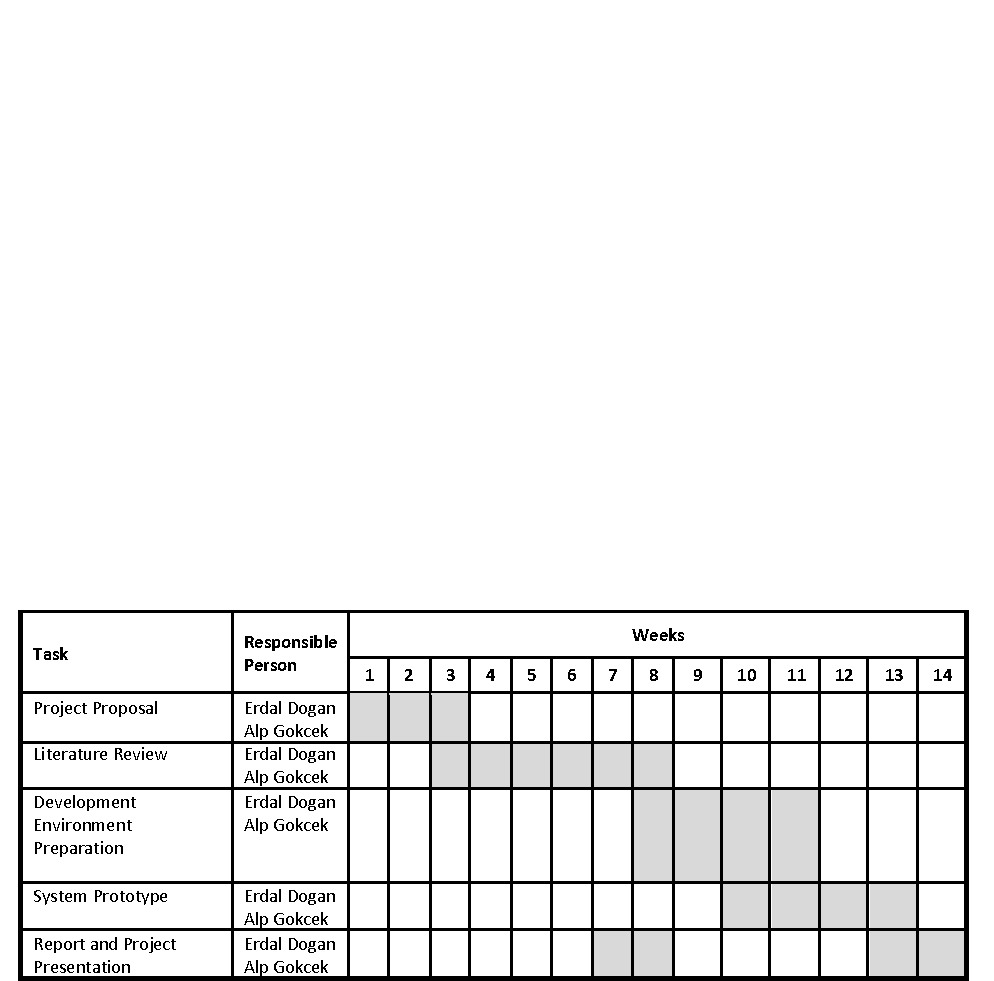
\includegraphics[width=\linewidth]{gantt}
	\end{table}
	\newpage
	\subsubsection{Aim of the project}
	Turkish Question Generation Model aims to fine-tune and train various state-of-art question generation models that are developed for other languages. Given a paragraph, passage or an entity in Turkish, it presents the possible questions that can be answered solely by the given content to the system.
	
	\begin{figure}[ht!]
		\centering
		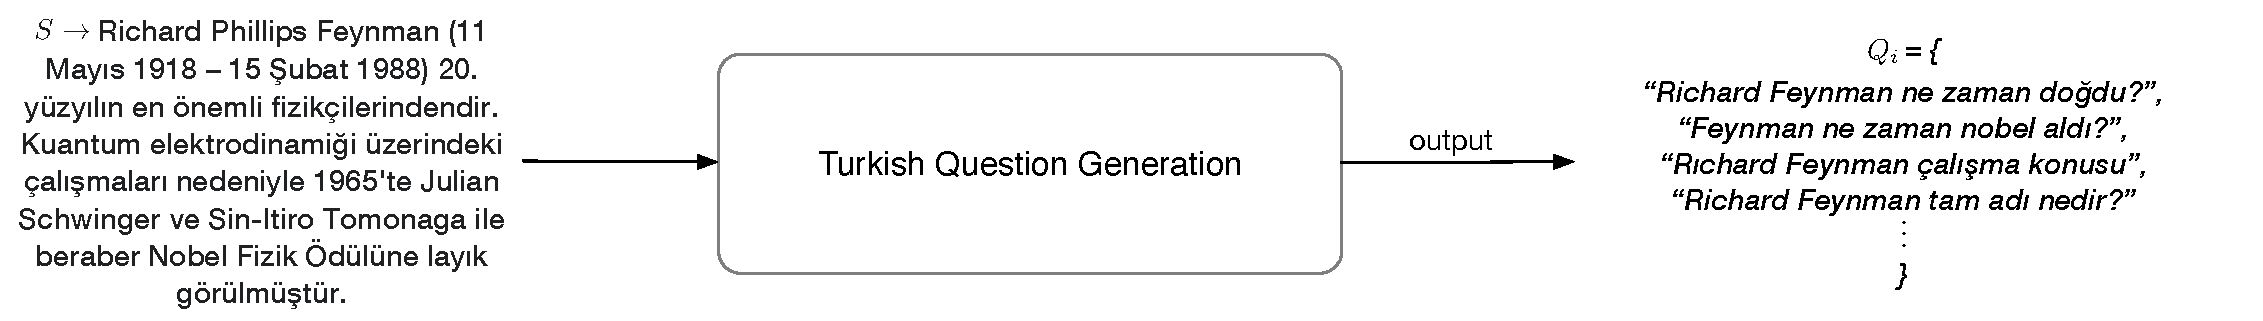
\includegraphics[scale=.37]{turkish_qg_system}
		\caption{Question Generation Model diagram}
	\end{figure}

	\gls{qg} models require extensively large training data. In this project, we have developed the  datasets for the development of the \gls{qg} model. Using our custom dataset, our aim is to compare performances of various models that we trained for Turkish Question Generation. 
	
	
	\subsubsection{Project Coverage}
	
	In the previous semester, construction of a data set for the training of \gls{qg} Model has been completed. Dataset consists of data which retrieved from the Turkish Wikipedia. \newline \par
	
	In this semester, we train several question generation models and fine tune if necessary for Turkish language with the dataset we had constructed. Later on, we aim to compare them regarding to common metrics such as BLEU \& ROGUE \footnote{See Section \ref{sc}} and present the results in detail. \newline \par
	
	The project's outcome will be a usable interface that users can pass paragraphs as input and retrieve the questions that has been generated automatically. Furthermore, a CLI\footnote{Command Line Interface} will be provided for other researchers to utilize in their workflows. 
	
	\pagebreak
	\subsubsection{Use Cases}
	Use case diagram of our project could be found in Figure \ref{usecases}. We have only one type of user at the moment. User will give a context paragraph to the system; then the system will return the questions generated from this context paragraph.
	\begin{figure}[ht!]
		\centering
		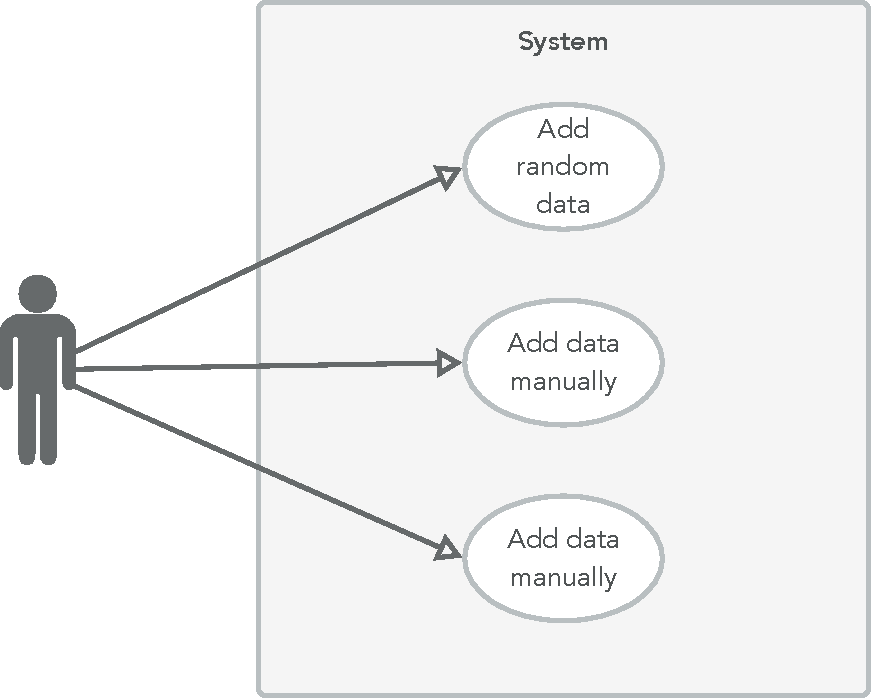
\includegraphics[width=0.5\textwidth]{use_case.pdf}
		\caption{Use case diagram of our QG system\label{usecases}}
	\end{figure}
	
	\subsubsection{Success Criteria}\label{sc}
	A couple of metrics will evaluate the outcomes of the project. Given that the outputs will be natural language instances, existing methods and algorithms specifically designed to evaluate generated natural language examples will be utilized. There are multiple algorithms and methods available, which consider different aspects of the outcome. Some of them are:
	\begin{itemize}
		\item BLEU
		\item ROUGE
		\item METEOR\\
	\end{itemize}
	
	Each of the enumerated methods takes different aspects into account, while \textit{BLEU} score is calculated with best match length is prominent, \textit{ROGUE} is based on recall score. They all have their tradeoffs, and neither of them is merely a strong indicator of success.
	
	\subsubsection{Project time and resource estimation}
	The project is estimated to take 16 weeks for two undergraduate students that are novices to the topic. While estimating, course load and other external factors are taken into account. The detailed timeline can be seen from Table 1 on the previous page. \\
	
	Assuming that each member spends 8 hours a week working on this project's issues, it makes approximately 128 hours per person, 256 hours spent in total. Also, it has been mentioned that computing resources will be required for the project. If we use cloud computing providers (AWS for this particular example) rates for this estimation, we observe that the hourly price is ~\$2 for a server that we need to run. Considering that these are very intensive applications, it might be the cases that the server will be up and making computations for long hours, 20 hours a week. This estimation sums up to \$600 in server running costs and 256 men hours. Notice that no access to books, online courses or any other learning material has not been included.
	
	
	\subsubsection{Solution Strategies and Applicable Methods}
	For the project, we decided to use off-the-shelf language models by fine-tuning them according to our data. We could have tried to achieve it without using such advanced models; however, there would be the risk of not completing the project in time or a flawed model could have been produced.
	
	\subsubsection{Risk Analysis}
	One of the significant risks that may occur is that the model gives questions that are not directly related to given inputs or contain grammatical/structural errors. There are not any risks.
	
	\subsubsection{Tools Needed}
	The project requires the development of Machine and Deep Learning Models from scratch. Due to wide selection of libraries for this purpose, the community behind it, and the de-facto standard of the AI research and scientific development, it has been decided that \textit{Python Programming Language} will be used for development and implementation during this project.\\
	
	Specifically, for the model development, an up-to-date, state-of-art library named \textit{PyTorch} will be used extensively. Also, the development of such models and processing large amounts of data requires computing resources. Therefore, servers configured with GPU optimization in mind will be required for a faster development process.
	
	
	
	\section{Theoretical Background}
	\subsection{Literature Survey}
	In this section, a survey of the literature from multiple sources could be found.
	\subsubsection{Question Answering}
	Question Answering (QA) automatically presents the answers to the question that users ask without any human interaction. In a QA model, it is expected that the system has access to the necessary information to answer the question.\\
	To develop such a model, we need extensive data consisting of Questions and their Answers, a duple that we will denote by <Q, A>. Unfortunately, labelling this kind of data manually or creating answers from scratch for an Artificial Intelligence based solution is not the most efficient.
	They address these problems by;
	\begin{enumerate}
		\item Large scale high-quality dataset from Community-QA websites such as Yahoo, Quora is obtained since they provide large scale QA pairs generated by real users.
		\item Two ways of accomplishing such task is implemented and compared. One is a retrieval-based method using Convolutional Neural Networks(CNN) and other is a generation-based method using Recurrent Neural Network (RNN).
		\item Outcomes of the QG model is integrated with end-to-end QA task. It is evaluated on three state-of-art datasets, SQuAD, MS MARCO, and WikiQA. Results show that generated questions can improve QA quality on all these three datasets.
	\end{enumerate}
	
	\begin{figure}[ht!]
		\centering
		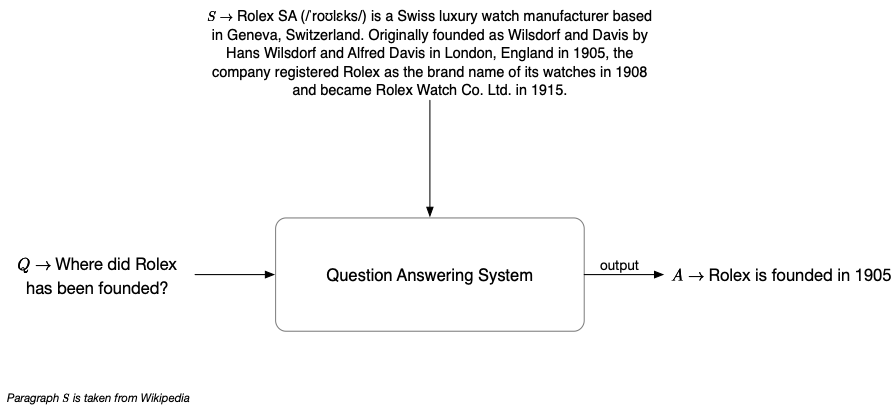
\includegraphics[scale=.8]{sample-qg}
		\caption{Sample Question Answering model}
	\end{figure}
	
	\subsubsection{Question Generation}
	Research engineers from Microsoft Research proposed extracting question from a given piece of text. \cite{duan2017question} While they used NLP methodologies and Neural Networks, they did not include the semantics of words in their paper.\\
	
	QG Engine is consist of four components:
	\begin{enumerate}
		\item Question Pattern Mining
		\item Question Pattern Prediction
		\item Question Topic Selection
		\item Question Ranking
	\end{enumerate}
	\subsubsection{BERT Language Model}
	We have encountered a language model called BERT, which is also known as Bidirectional Encoder Representation from Transformers developed by Google \cite{vaswani2017attention}. It uses a machine learning model called Transformers. We have researched other language models, and for the language translation problem, we have found two techniques which are LSTM and Transformers.\\
	
	First of all, we have found out that LSTMs are slow to train, words are passed sequentially, and words are getting generated sequentially which can take significant time for the neural network to learn the language. Furthermore, LSTMs are not truly bidirectional; they learn left-to-right and right-to-left separately and concatenate afterwards. Thus, a need for  Transformers arose. Transformers are faster because they can process words simultaneously and deeply bidirectional since they can learn in both directions. \\
	
	On Figure \ref{transformer}, you can see the architecture of a transformer. It is formed by two components which are encoder and decoder.\\
	\begin{figure}[ht!]
		\centering
		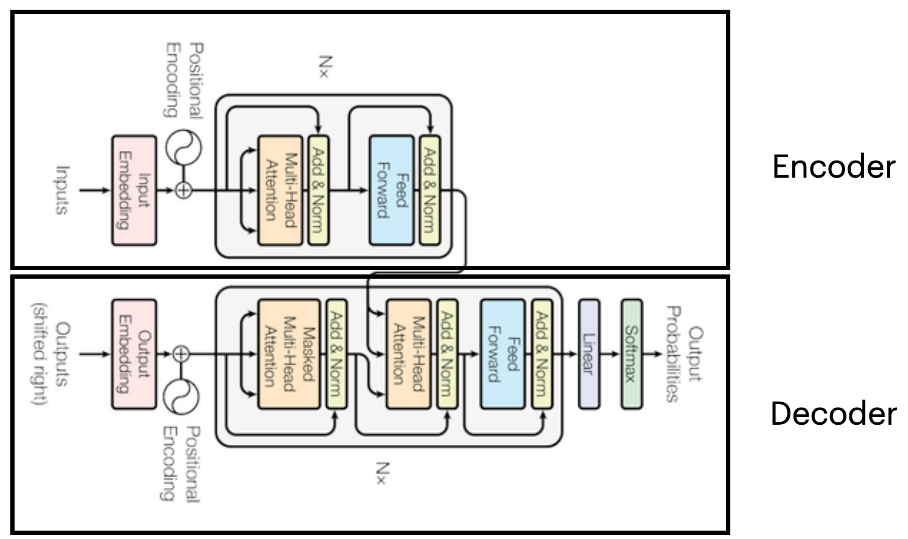
\includegraphics[scale=.8]{transformers}
		\caption{Architecture of a \textit{Transformer}\label{transformer}}
	\end{figure}
	
	As the BERT's name suggests, we will obtain the BERT language model if we put encoders on after another. The architecture of the BERT language model could be found in figure \ref{bert-architecture}. It is the current state-of-the-art language model for NLP tasks. \cite{chan-fan-2019-recurrent}
	
	\begin{figure}[ht!]
		\centering
		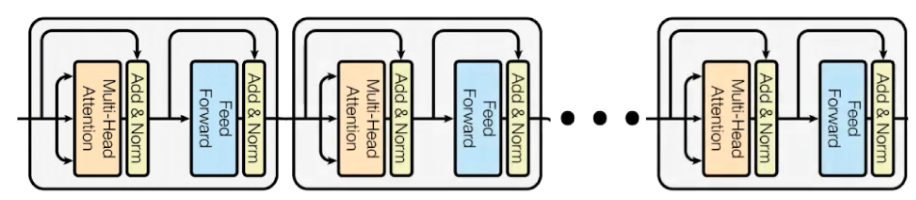
\includegraphics[scale=.8]{bert-model-architecture}
		\caption{BERT language model architecture\label{bert-architecture}}
	\end{figure}
	We have found a paper that uses this language model to solve our problem, and they have made sequentially improved three models which are BERT-QG (BERT Question Generation), BERT-SQG (BERT Sequential Question Generation) and BERT-HLSQG (BERT Highlight Sequential Question Generation) models. QG is the simplest model that this paper introduces. It is the initial attempt to create a powerful Question Generation Model using BERT. As proposed by researchers, considering the previous decoded results significantly improve the quality of the model. However, in BERT-QG, token generation is performed without considering the previous states or decoded results. Due to this consideration, BERT-SQG is developed. BERT-SQG addressed the problem of ignoring the previous decodes in the BERT-QG model. However, researchers researched and concluded that BERT-SQG is not capable of producing quality questions in lengthy situations, and if an answer phase appears multiple times, it struggles to decide which one to decide. As a result, BERT-SQG is restructured, and BERT-HLSQG, a model outperforming BERG-SQG is obtained.\\
	
	They have compared these models with the known to be the best question generation models which were NQG-RC and PLQG. NQG-RC is a seq2seq question model based on bidirectional LSTMs. PLQG is a seq2seq network which is capable of handling long text input. This model is known to be the state-of-the-art models for QG tasks. As shown in table \ref{recurrent-comparison}, their models have outperformed the state-of-the-art models on every metric.\\
	\begin{table}[ht!]
		\caption{Performance comparison of Question Generation models on different datasets\label{recurrent-comparison}}
		\centering
		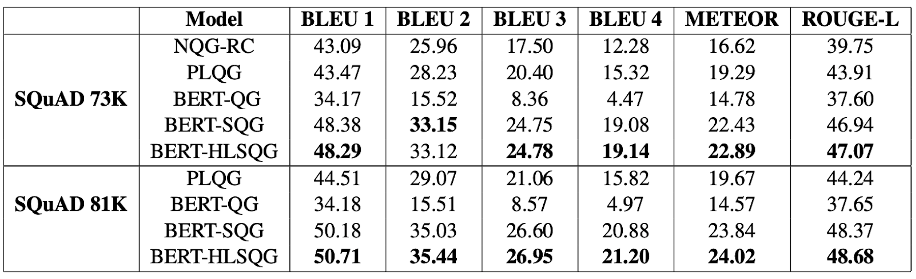
\includegraphics[scale=.7]{recurrent-comparison}
	\end{table}
	
	\subsection{Question Generation Model with BERT Language Model}
	As a result of this literature survey, we have decided to go with the BERT language model. BERT language model shows significant performance over various NLP tasks, such as classification, summarization, translation. It has a robust architecture behind it which is transformers. We have searched a pre-trained Turkish model of BERT, and we found a repository on GitHub for it. Starting from next week, we will start using this model as well.\\
	
	As for the dataset, we have decided to go with Turkish Wikipedia dataset. Since the data of Wikipedia is close to textbook data, it should be beneficial to train our model with this dataset. Moreover, our advisor, Seniz Demir, had a Wikipedia Parser project. Thus, we will use the Turkish Wikipedia dataset.
	
	
	
	\section{Analysis and Modeling}
	\label{refhere}
	Aim of this project is to develop a Turkish Question Generation Model using our custom dataset. Given a paragraph or a piece of text, our model creates the possible questions that can be answered with the information given in that paragraph. \newline \par
	
	However, such a model's development requires an extensively large and labelled dataset consisting of paragraphs, related questions, and answers to those questions. Unfortunately, such dataset is not available in the Turkish language. There are examples of it, but they neither contain large amounts of the information nor find the data reliable. \newline \par
	
	For the reasons described above, we composed our dataset in previous semester. Our dataset consists of paragraphs from Turkish Wikipedia. Using the Turkish Wikipedia's Person entities, we created the question patterns regarding to specification of the Person's in dataset. Later, these questions patterns are completed by substituting the person's name with the placeholders. As a result, we obtained formal question-answer pairs along with the paragraphs. \newline \par
	
	However, we must also confirm that the answer to the question is also found in the paragraph. For this reason, we use a fuzzy search algorithm in order to determine if the answer is in the paragraph or not. If so, we add the questions to our dataset, if not, we skip to the next question. \newline \par
	
	
	
	\subsection{System Factors}
	Since our work is based on the data acquired from Wikipedia and its manipulation, source data is highly influential on the outcome. While creating the dataset, we always aim to create grammatically flawless questions while covering the variety of inputs that may come from the end-user
	
	\subsection{How System Works}
	Input data consists of ~53,000 person entities from Turkish Wikipedia. Occupations of each person and their attributes are also presented. For instance, for a 'Soldier', given attributes are: 'Rank', 'Wars', 'Nationality', 'Commanders' etc. Given that most of these attributes are also mentioned in the corresponding person's description paragraph, when we create the questions that ask about these attributes, we will have the description paragraph and the questions together. 
	
	Initially, each question patterns for attributes are created manually containing a placeholder for the person's name. Later, by iterating over each person and substituting names for their attributes, we create example questions. 
	
	When we iterate over every person, we accumulate a dataset consisting of paragraphs that describe the person and questions about the person's attributes, which is also contained in the paragraph.  
	
	\subsubsection{Modelling}
	
	The system can be inspected under two groups; Dataset Production and Development of the Question Generation Model. \newline \par
	
	Figure 6 shows the relationship between person entities, their attributes and the question patterns. Each person has a set of attributes, and each attribute has a set of question patterns. \newline \par
	
	\begin{figure}[h]
		\centering
		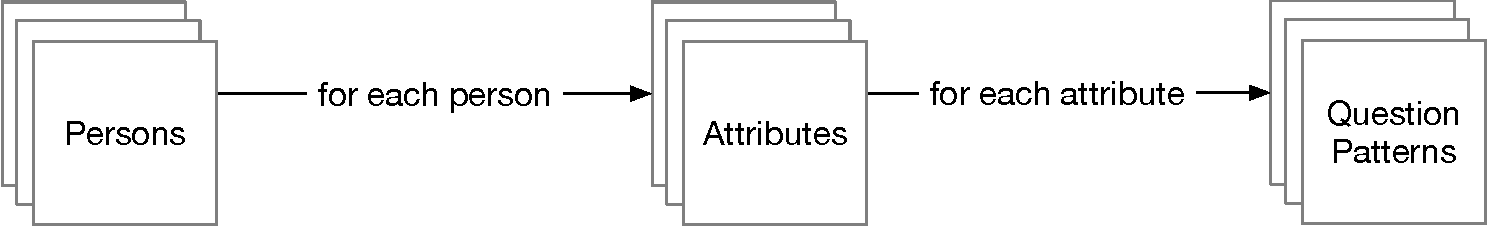
\includegraphics[scale=.5]{architecture.pdf}
		\caption{System Entities\label{per-attr-qp}}
	\end{figure}
	
	
	
	Figure 7 shows the relationship between an attribute and the questions. For an attribute, there are multiple question patterns. When the questions are generated using the pattern, cumulatively these patterns create questions about the person's attribute. \newline \par
	
	\begin{figure}[h]
		\centering
		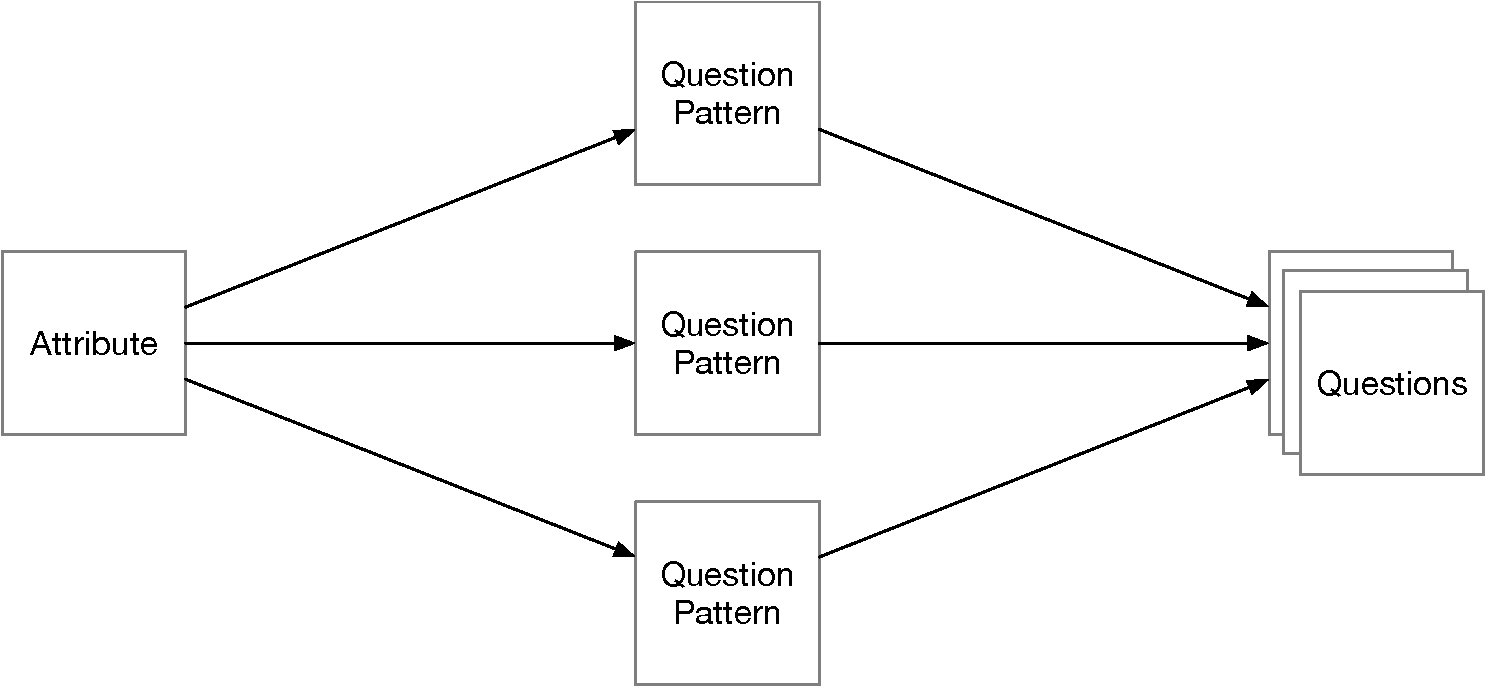
\includegraphics[scale=.5]{attr_questions.pdf}
		\caption{Relationship of an attribute to Questions\label{attr-qg}}
	\end{figure}
	
	
	Figure 8 shows the relationship between the person entity and how the output data for a single person is generated. Each person has a descriptive paragraph and set of attributes. These attributes yield to set of questions that the description paragraph can answer. When the paragraph and the questions are coupled together, we get a paragraph-questions pair for our dataset. \newline \par
	
	\begin{figure}[h]
		\centering
		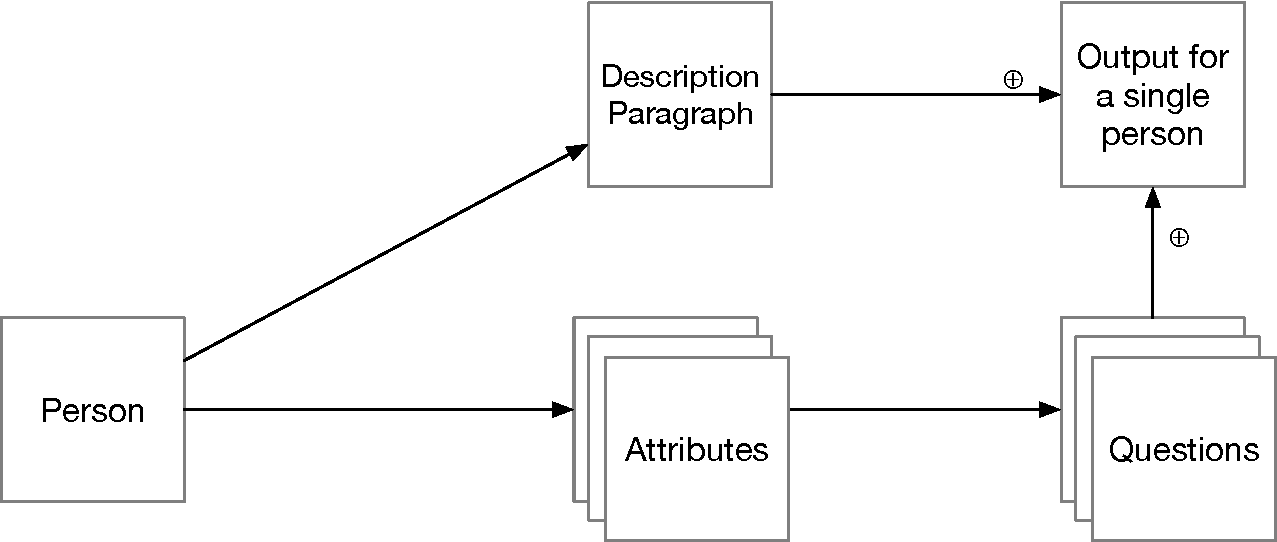
\includegraphics[scale=.5]{person_output.pdf}
		\caption{Relationship of an attribute to Questions}
	\end{figure}
	
	\newpage
	\subsubsection{System Architecture }
	Explanation of system architecture.
	\begin{figure}[h!]
		\centering
		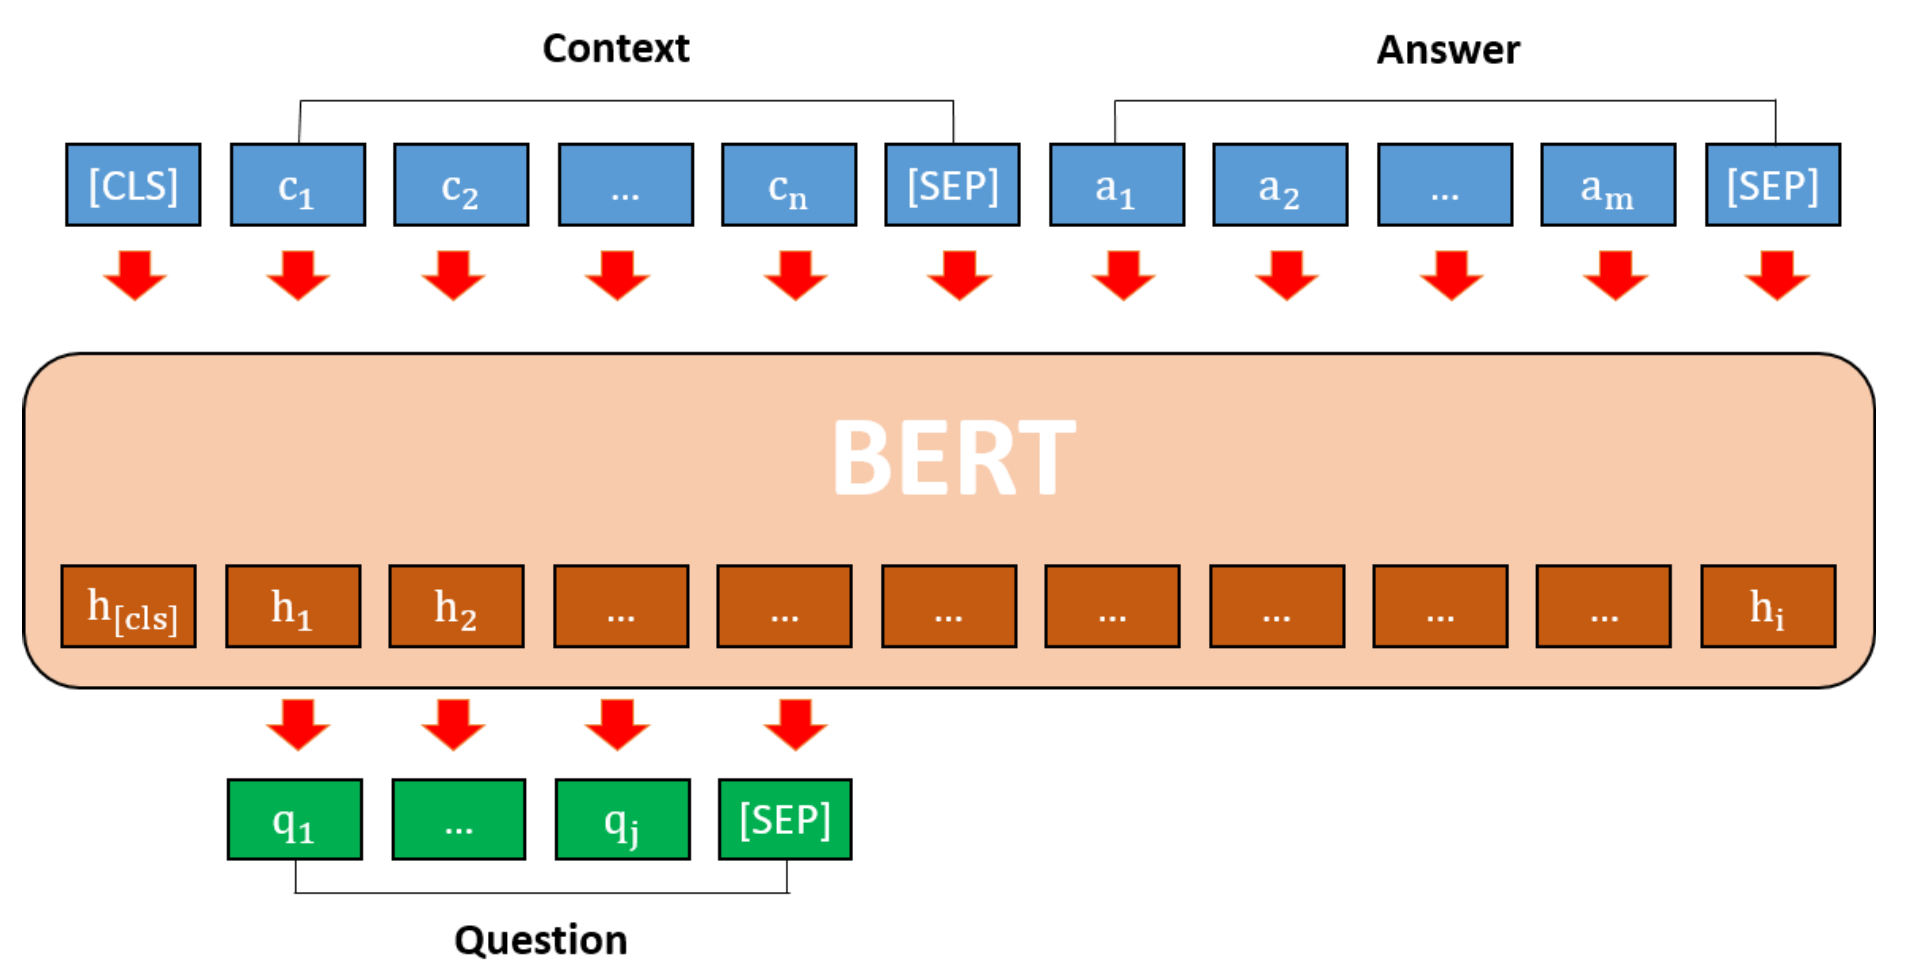
\includegraphics[width=0.75\textwidth]{bert-qg.png}
		\caption{BERT-QG Architecture \cite{chan-fan-2019-bert}\label{bertqg-arch}}
	\end{figure}
	
	\subsubsection{UML (Unified Modeling Language) Diagrams}
	UML Diagrams can be seen from Appendix C
	
	\section{Design, implementation and testing}
	During the design phase of our project, we had two different components that have to be completed. These are:
	\begin{itemize}
		\item A Turkish question answering dataset will be used to train the \gls{qg} model.
		\item A \gls{qg} model.
		\item User-Interface
	\end{itemize}
	This section will explain the design process we have followed during the design, implementation, and testing of these two components separately.
	\subsection{Design}
	\subsubsection{Dataset}\label{dataset-design}
	Before creating our dataset, we have researched if any of the datasets are suitable and sufficient. We have found one dataset that is suitable for our model. That dataset has around 2.2k questions, and the descriptive texts were about Turkish \& Islamic Science History, which is not completely suitable and sufficient. Hence, we have decided to create our dataset. During the design phase of the dataset, we have used 2 Wikipedia datasets. The first data was semi-cleaned scrapped Turkish Wikipedia data. Data we had has the short descriptions and the table contents. An example of the table content could be found in Figure \ref{wiki-table-content}. 
	\begin{figure}[h!]
		\centering
		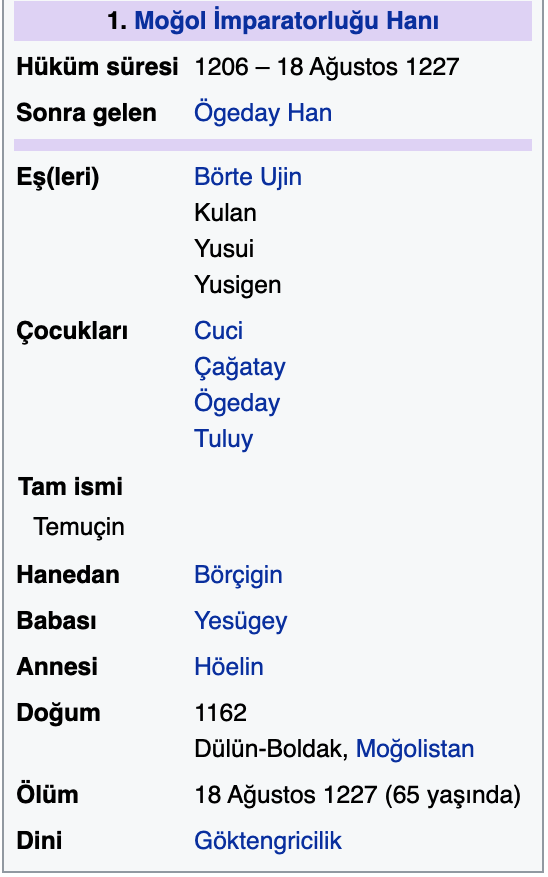
\includegraphics[scale=.3]{wiki-table-content}
		\caption{Sample Wikipedia table content\label{wiki-table-content}}
	\end{figure}
	
	However, this data was insufficient for our dataset since most of the table contents' data does not appear in the short description. Thus, we had to use long descriptions for each of them. After that, we also matched the whole Wikipedia Turkish dump we found from Kaggle with our first data. This data had long descriptions of every document that is currently available on Wikipedia. During the matching phase, we have decided to match each document by their id's.\\
	
	After finishing the data part, we have started to analyze our data. We have grouped each person according to their occupation. After grouping, we have found out that we have twenty different occupations. Each occupation has its table attributes. Our main goal is to generate question patterns according to their occupations and the most used ten attributes for that specific occupation. Our analysis on the Wikipedia persons data could be found in Appendix A.\\
	
	Finally, we have started to generate the question patterns according to the occupation and the attributes. During this process, we have decided to the question pattern styling.\\
	
	\subsubsection{Question Generation Model}\label{qgmodel-design}
	As discussed in Section \ref{refhere}, we train various models for Question Generation task. This models are designed for other languages than Turkish. In this part of the project, our aim is train these models for Turkish while preserving their high performance scores. \newline \par
	
	\subsubsection{Question Generation Model}\label{qgmodel-design}
	In the design process of Question Generation Model, we have followed the architecture of the \cite{chan-fan-2019-recurrent}. For the given paragraph $C=[c_1, c_2, ..., c_n]$, the answer phase $A=[a_1, a_2, ..., a_n]$ and the question $\hat{Q} = [\hat{q_1}, ..., \hat{q_i}]$, the input sequence $X$ will be shown as follows.
	\begin{equation}
	X =  ([CLS], C, [SEP], A, [SEP])\label{formula1}
	\end{equation}
	
	There are two different tokens in that sequence. These can be summarized as follows:
	\begin{itemize}
		\item \textit{$[CLS]$}: Token shows the beginning of a sequence.
		\item \textit{$[SEP]$}: Token separates the answer from the context and the generated question.
	\end{itemize}
	Assume that $BERT()$ is the BERT language model and initially, we obtain the hidden representation $ \textbf{H} \in {R}^{|X| x h}$ by $\textbf{H} = BERT(X)$, where $|X|$ is the length of the input sequence, $h$ is the size of the hidden dimension. Then, $H$ is passed to a dense layer $\textbf{W} \in {R}^{|X| x V}$ followed by the the softmax function shown in Equation \ref{softmax} and \ref{argmax}.
	

	\begin{equation}
	Pr(w|x_i) = softmax(\textbf{h} \cdot \textbf{W} + \textbf{b}), \forall {x}_{i} \in X \label{softmax}
	\end{equation}
	\begin{equation}
	\hat{q_i} = argmax_{w}Pr(w|x_i)\label{argmax}
	\end{equation}
	The softmax is applied along the dimension of the input sequence. All of the parameters of BERT language model and $W$ are fine-tuned jointly to maximize the logarithmic probability of the correct token $\hat{q_i}$. A sequence of tokens $[w_1, ..., w_{|x|}]$ is generated and we use the first generated \textit{$[SEP]$} symbol as the end of the generated question. 

	\subsection{Implementation}
	Similar to the design part, we have developed and implemented each component separately. We have implemented these components with the Python Programming Language.
	\subsubsection{Dataset}
	While creating the dataset, we first created our entity classes according to the data we have. The classes have been created according to the data could be found in Figure \ref{fig:dataset_person} and Figure \ref{fig:dataset_persondataparser}.\\
	
	As mentioned in Section \ref{dataset-design}, we have already decided on the question patterns on the designing phase. In the implementation phase, we have generated around 700 question patterns manually. Sample question patterns that we have generated could be found in Figure \ref{qg-patterns}. Complete list is provided in Appendix B.
	\begin{figure}[h!]
		\centering
		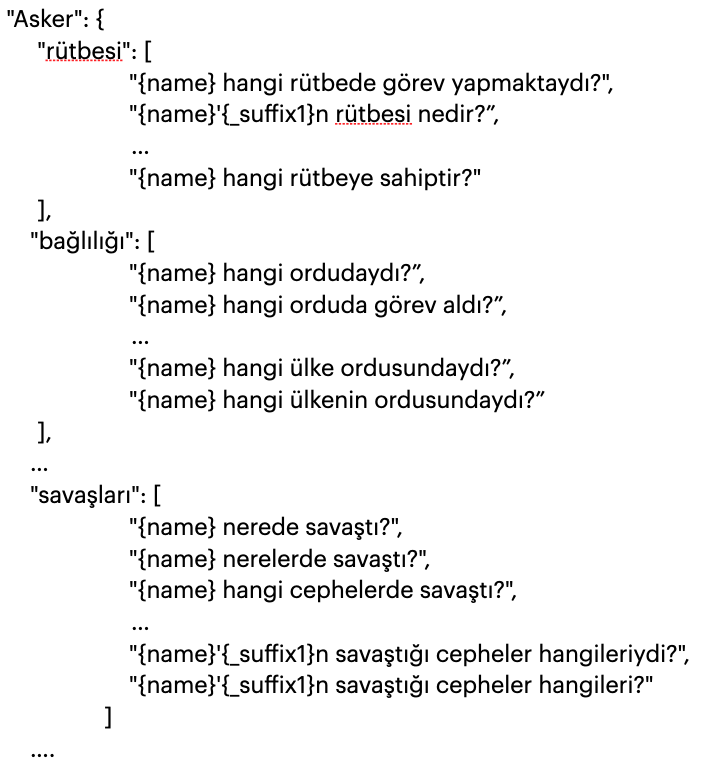
\includegraphics[scale=.5]{qg-patterns}
		\caption{Sample Question Generation patterns\label{qg-patterns}}
	\end{figure}
	After generating the question patterns, we needed to ensure the feature (answer of the question) is included in the context (description paragraph). To address this issue, we used a fuzzy search mechanism while searching an attribute in the long description. We have researched and found out that in fuzzy search algorithms, the Lavensthein's distance formula. After that, we found a package that is the implementation of that formula called \textit{fuzzywuzzy}. We pass the long description, and the answer that we want to generate a question from then the method calculates the similarity in the range of 0-1. We have decided to use 0.6 as the threshold. If the ratio is higher than our threshold value, then we generate the questions. In Figure \ref{ilker-basbug}, the questions that have been generated for Ilker Basbug, who is the 26th Chief of the General Staff of Turkey, can be seen. Wikipedia classified him as a army officer, thus, we have generated the possible questions using the data from the table. We name our dataset as TurQuAd.\\
	
	\begin{figure}[h!]
		\centering
		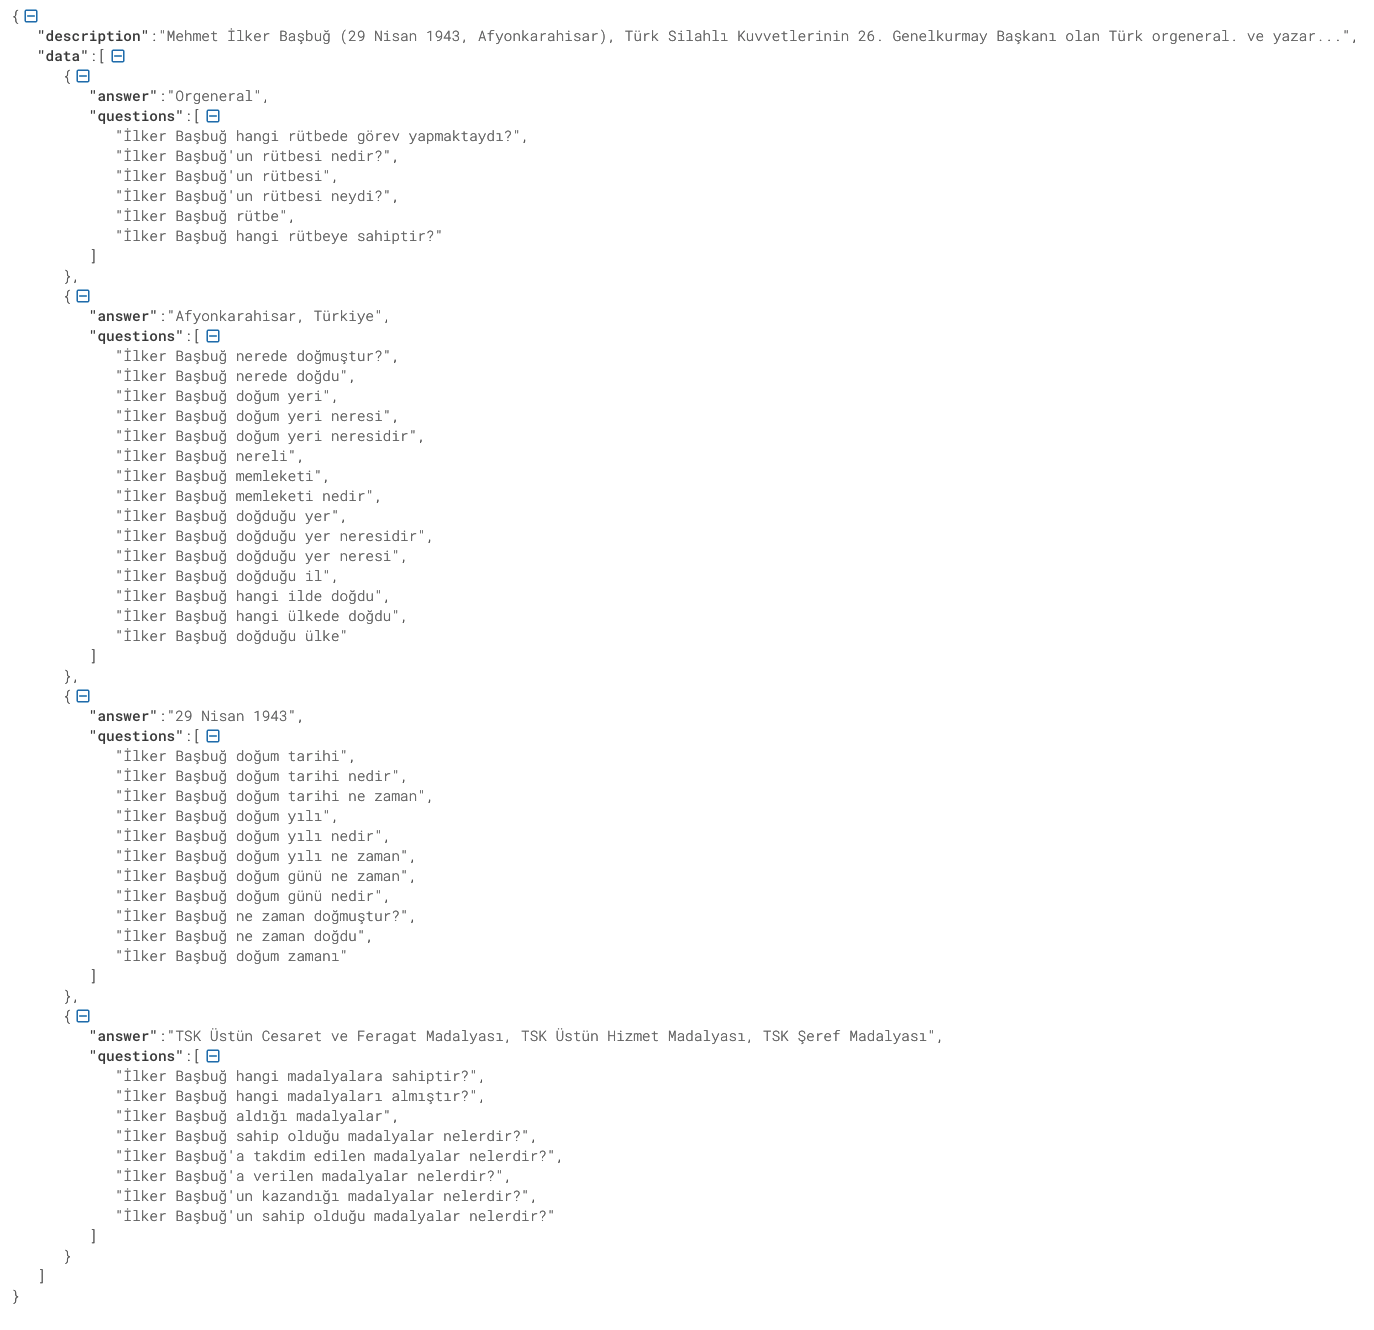
\includegraphics[scale=.3]{ilker-basbug}
		\caption{Questions generated for Ilker Basbug (26th Chief of the General Staff of Turkey)\label{ilker-basbug}}
	\end{figure}
	
	
	Another critical aspect of the implementation part was the performance. There were around 53,000 people in the data, and the whole Wikipedia data is approximately 500 MB. Our computers were not sufficient for this processing so we have decided to use cloud services. We have used our previous knowledge on multiprocessing from Operating Systems and tweaked our code to work with multiple CPU's in parallel.	
	\subsubsection{Question Generation Model}
	In the last semester, we constructed our custom dataset in a format that is similar to famous SQuAD \cite{rajpurkar2016squad} dataset. Given that most of the question generation models, along with the BERT Language model, are built on top of and highly compatible with SQuAD dataset, we aim to format our TurQuAd dataset as closely as possible. \newline \par 
	
	We have made a comprehensive research on several open-source Question Generation projects and worked on creating our QG model. During our research, we have found out that most of the state-of-art models are developed by using BERT language model. However, our main goal was to develop the QG model for the Turkish language. There are existing pre-trained language models based on BERT for Turkish language such as BERTurk \cite{stefan_schweter_2020_3770924}. We utilized the pretrained models on this project.
	\newline \par 
	
	We use the PyTorch Framework to train our QG Models based on BERT Language Model. The pretrained model uses 512 hidden dimensions, and 512 attention size. Dropout probability is set to 0.1 between layers. The Adam Optimizer is applied during the training process, with an cross entropy loss function and initial learning rate of 5e-5. The batch size for the update is set as 28. Our models used a single NVIDIA Tesla K80 GPUs on Microsoft Azure VMs\footnote{Standard NC6 Promo Instance} for 3 epochs training. 
	\subsubsection{Tokenization}
	A tokenizer is in charge of preparing the inputs for a model. There are 3 different key features of the tokenizers. These are:
	Splitting strings in sub-word token strings, converting tokens strings to ids and back, and encoding/decoding
	Adding new tokens to the vocabulary in a way that is independent of the underlying structure which helps the model to learn unknown inputs easier
	
	Managing special tokens (like mask, beginning-of-sentence, etc.): adding them, assigning them to attributes in the tokenizer for easy access and making sure they are not split during tokenization.
	
	\begin{figure}[h!]
		\centering
		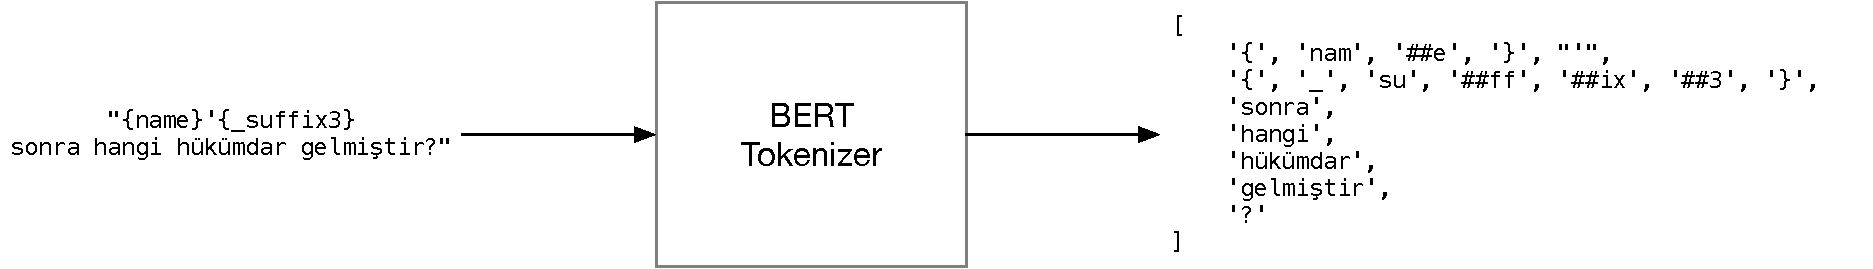
\includegraphics[width=\textwidth]{tokenization.pdf}
		\caption{Tokenization example\label{token}}
	\end{figure}
	
	\subsubsection{Delexicalization}
	Delexicalization is the process that replacing language-specific words with language-agnostic meaning. Delexicalization can be used for anonymization (e.g., removing proper names) or to improve the performance of an NLP application by removing over-specific phrases (numericals, named entities, names, etc). After the generation of the questions, we are replacing the placeholders with the correct token. We have generated a delexicalized version of our dataset. We will mention the effect of the delexicalization on results in following sections.
	
	\begin{figure}[h!]
		\centering
		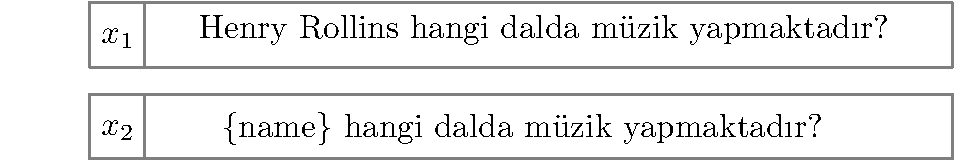
\includegraphics[scale=.6]{delex.pdf}
		\caption{Non-Delexicalized ($x_1$) vs Delexicalized ($x_2$) sentences)\label{delex}}
	\end{figure}

	\subsubsection{Output Examples}
	Questions produced by our system, after placing the names in the placeholders as a result of delexicalization process, can be seen below against the ground truths. 
	\newline
	
	\noindent
	\fbox{\parbox{\textwidth}{\textbf{Ground Truth:} Erkin Koray aktif yılları nelerdir?\newline
			\textbf{Prediction:} Erkin Koray hangi yıllarda müzisyenlik yapmıştı?}}
	\newline
	
	\noindent
	\fbox{\parbox{\textwidth}{\textbf{Ground Truth:} Alex De Souza'nın maçlardaki pozisyonu nedir?\newline
		\textbf{Prediction:} Alex De Souza hangi mevkiide oynamaktadır?}}		
	\newline

	\noindent
	\fbox{\parbox{\textwidth}{\textbf{Ground Truth:} Orhan Pamuk hangi ödülleri almıştır?\newline
			\textbf{Prediction:} Orhan Pamuk'a takdim edilen ödüller nelerdir?}}		
	\subsubsection{GUI}
	We had to create a GUI so that users of our system can use our model easily. Before creating the GUI, we have decided to make a web application to develop a web application to reach many users. In this context, we needed a front-end and a back-end application. For the frontend, we used the React.js library developed by Facebook, which many companies around the world use in addition to Javascript. We have tried to design a simple, clear user interface. The design of our frontend application could be found in Figure \ref{ui}. 
	
	\begin{figure}[h!]
		\centering
		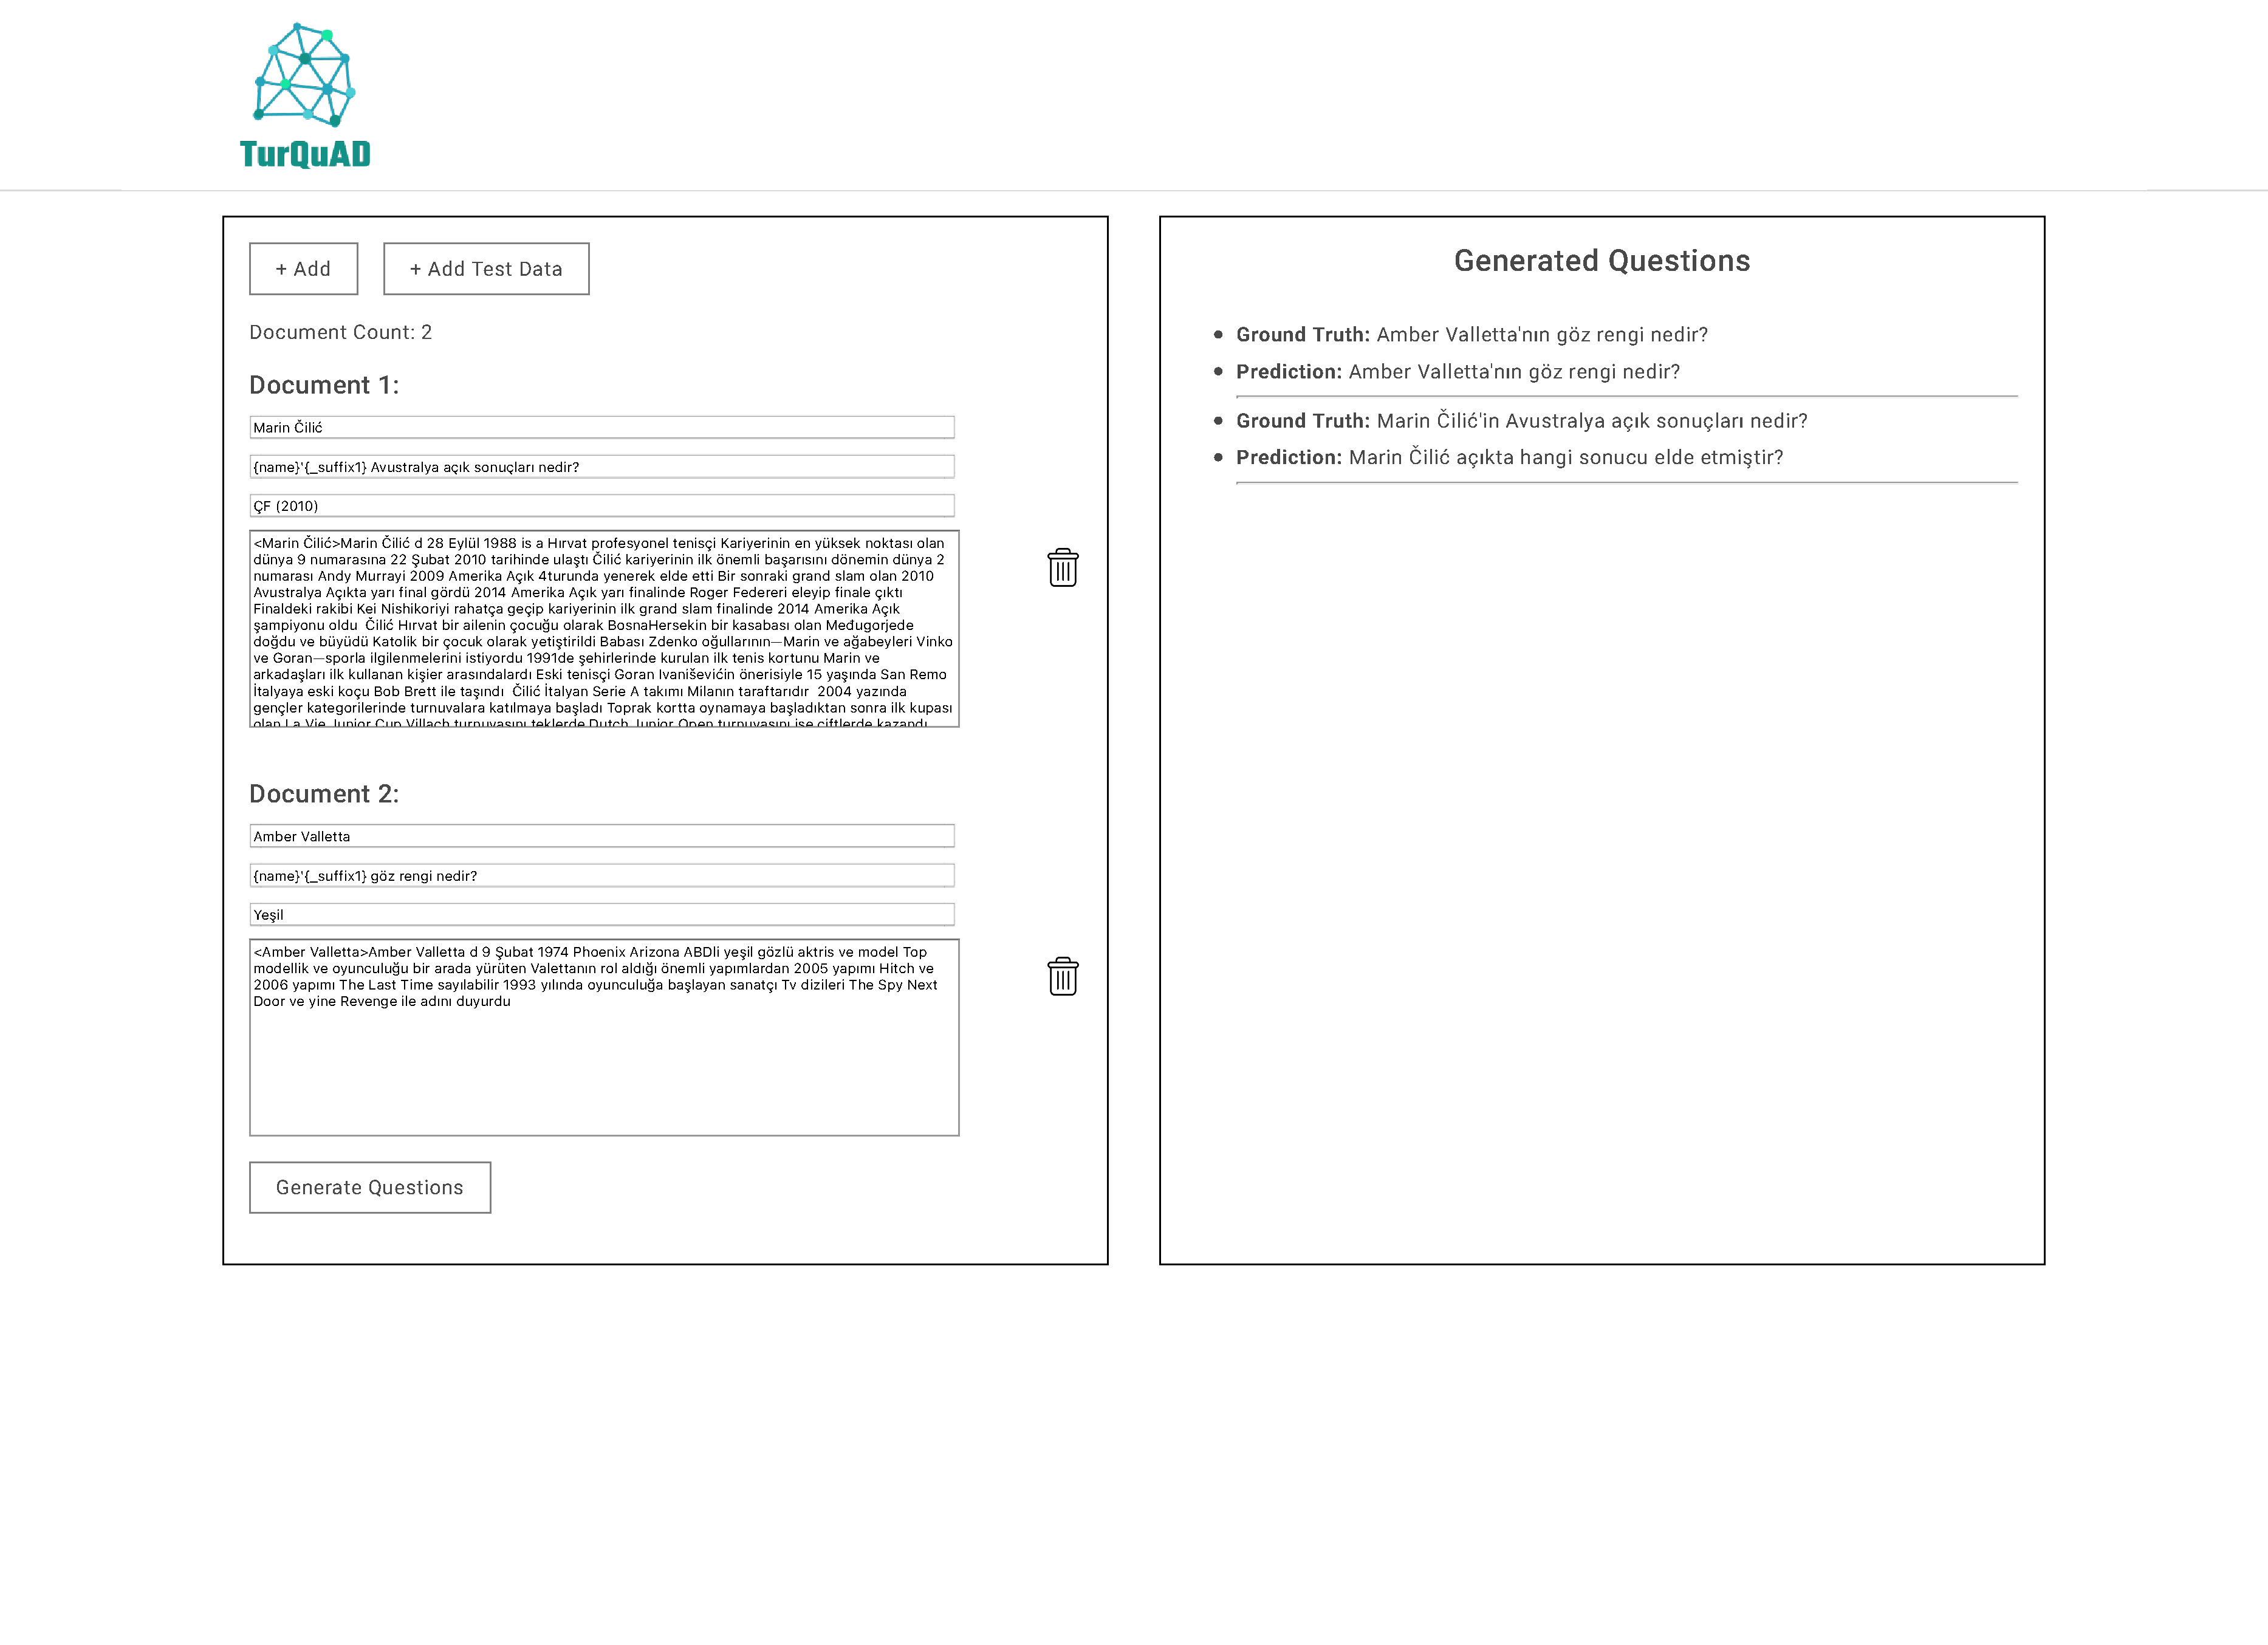
\includegraphics[width=\textwidth]{ui.pdf}
		\caption{User interface design of our frontend application}
		\label{ui}
	\end{figure}
	
	There were three different scenarios in our application and these were Add Data, Add Random Test Data and Generate Questions. We have created one panel for adding the data and one panel for showing the generated questions. Besides that, we have added four different call-to-action buttons in adding a data panel to cover these cases. We have connected the frontend application with the backend application with two endpoints. One endpoint is for gathering random test data, and the other endpoint is for generating questions. After generating data through the UI, data is sent to the backend application.
	\newline \par
	For the backend, we used the library called Flask, which makes it easy for us to create a REST API in Python. The main reason we preferred Flask was that the QG Model we have created was developed with the Python language. After the request is received for the method of generating questions, the backend application preprocesses the JSON payload for the model. After the preprocessing phase, the deep learning model generates the questions and returns them through the backend application.
	
	\subsection{Testing}\label{eval}
	BLEU or in longer version BiLingual Evaluation Understudy, is a metric for automatically evaluating machine-translated text. The BLEU score is a number between zero and one that measures the similarity of the machine-translated text to a set of high-quality reference translations. A value of 0 means that the machine-translated output has no overlap with the reference translation in other words it is a low-quality output while a value of 1 means there is perfect overlap with the reference translations which means a high-quality output. It has been shown that BLEU scores correlate well with human judgment of translation quality. Note that even human translators do not achieve a perfect score of 1.0. It is the N-gram precision and aims to find what percentage of machine n-grams can be found in the reference translation.
	\newline \par 
	\begin{figure}[h!]
		\centering
		\includegraphics[width=\textwidth]{bleu_table.pdf}
		\caption{BLEU Score Table (scale 0-100)}
	\end{figure}
	
	\begin{table}[htb!]
		\centering
		\caption{Evaluation results. Whole Paragraph, Non-Delexicalization}
		\begin{tabular}{l | l | l | l | l | l | l}
			&       & \multicolumn{2}{l}{Validation}\vline                                                                                & \multicolumn{2}{l}{Train}    \vline                                                                                   &                                                      \\
			\hline
			& BLEU  & \begin{tabular}[c]{@{}l@{}}Sentence\\ Loss\end{tabular} & \begin{tabular}[c]{@{}l@{}}Word\\
				Loss\end{tabular} & \begin{tabular}[c]{@{}l@{}}Sentence\\ Loss\end{tabular} & \begin{tabular}[c]{@{}l@{}}Word\\ Loss\end{tabular} & \begin{tabular}[c]{@{}l@{}}Train\\ Loss  \end{tabular} \\ \hline
			Epoch 1 & 0.327 &
			67.563                                                 & 5.753                                           & 52.255                                                  & 4.521                                               & 4.771                                                \\
			Epoch 2 & 0.314 & 72.211                                                  & 6.161                                               & 33.405                                                   & 2.909                                               & 3.001                                                \\
			Epoch 3 & 0.325 & 77.203                                                  & 6.570                                               & 23.486                                                   & 2.016                                               & 2.164                                               
		\end{tabular}
		\label{manual}
	\end{table}
	
\begin{table}[htb!]
	\centering
	\caption{Evaluation results. Whole Paragraph, Delexicalization}
	\begin{tabular}{l | l | l | l | l | l | l}
		&       & \multicolumn{2}{l}{Validation}\vline                                                                                & \multicolumn{2}{l}{Train}    \vline                                                                                   &                                                      \\
		\hline
		& BLEU  & \begin{tabular}[c]{@{}l@{}}Sentence\\ Loss\end{tabular} & \begin{tabular}[c]{@{}l@{}}Word\\
			 Loss\end{tabular} & \begin{tabular}[c]{@{}l@{}}Sentence\\ Loss\end{tabular} & \begin{tabular}[c]{@{}l@{}}Word\\ Loss\end{tabular} & \begin{tabular}[c]{@{}l@{}}Train\\ Loss  \end{tabular} \\ \hline
		Epoch 1 & 0.512 & 25.223                                                  & 1.632                                               & 14.323                                                  & 0.921                                               & 1.156                                                \\
		Epoch 2 & 0.523 & 24.647                                                  & 1.553                                               & 8.051                                                   & 0.527                                               & 0.629                                                \\
		Epoch 3 & 0.527 & 26.744                                                  & 1.763                                               & 9.135                                                   & 0.606                                               & 0.548                                               
	\end{tabular}
\label{wp}
\end{table}

\begin{table}[htb!]
	\centering
	\caption{Evaluation results. First Paragraph, Delexicalization}
	\begin{tabular}{l | l | l | l | l | l | l}
		&       & \multicolumn{2}{l}{Validation}\vline                                                                                & \multicolumn{2}{l}{Train}    \vline                                                                                   &                                                      \\
		\hline
		& BLEU  & \begin{tabular}[c]{@{}l@{}}Sentence\\ Loss\end{tabular} & \begin{tabular}[c]{@{}l@{}}Word\\
			Loss\end{tabular} & \begin{tabular}[c]{@{}l@{}}Sentence\\ Loss\end{tabular} & \begin{tabular}[c]{@{}l@{}}Word\\ Loss\end{tabular} & \begin{tabular}[c]{@{}l@{}}Train\\ Loss  \end{tabular} \\ \hline
		Epoch 1 & 0.503 & 26.452                                                  & 1.769                                               & 13.427                                                  & 0.871                                               & 1.155                                                \\
		Epoch 2 & 0.525 & 22.906                                                  & 1.553                                               & 9.132                                                   & 0.585                                               & 0.633                                                \\
		Epoch 3 & 0.521 & 26.103                                                  & 1.722                                               & 8.568                                                   & 0.877                                               & 0.550                                               
	\end{tabular}
\label{fp}
\end{table}

\begin{table}[htb!]
	\centering
	\caption{Evaluation results. Last Paragraph, Delexicalization}
	\begin{tabular}{l | l | l | l | l | l | l}
		&       & \multicolumn{2}{l}{Validation}\vline                                                                                & \multicolumn{2}{l}{Train}    \vline                                                                                   &                                                      \\
		\hline
		& BLEU  & \begin{tabular}[c]{@{}l@{}}Sentence\\ Loss\end{tabular} & \begin{tabular}[c]{@{}l@{}}Word\\
			Loss\end{tabular} & \begin{tabular}[c]{@{}l@{}}Sentence\\ Loss\end{tabular} & \begin{tabular}[c]{@{}l@{}}Word\\ Loss\end{tabular} & \begin{tabular}[c]{@{}l@{}}Train\\ Loss  \end{tabular} \\ \hline
		Epoch 1 & 0.502 & 31.758                                                  & 2.046                                               & 13.701                                                  & 0.882                                               & 1.135                                                \\
		Epoch 2 & 0.501 & 25.602                                                  & 1.608                                               & 9.698                                                   & 0.631                                               & 0.634                                                \\
		Epoch 3 & 0.524 & 22.875                                                  & 1.506                                               & 8.593                                                   & 0.568                                               & 0.572                                               
	\end{tabular}
\label{lp}
\end{table}

\begin{table}[htb!]
	\centering
	\caption{Evaluation results. Middle Paragraph, Delexicalization}
	\begin{tabular}{l | l | l | l | l | l | l}
		&       & \multicolumn{2}{l}{Validation}\vline                                                                                & \multicolumn{2}{l}{Train}    \vline                                                                                   &                                                      \\
		\hline
		& BLEU  & \begin{tabular}[c]{@{}l@{}}Sentence\\ Loss\end{tabular} & \begin{tabular}[c]{@{}l@{}}Word\\
			Loss\end{tabular} & \begin{tabular}[c]{@{}l@{}}Sentence\\ Loss\end{tabular} & \begin{tabular}[c]{@{}l@{}}Word\\ Loss\end{tabular} & \begin{tabular}[c]{@{}l@{}}Train\\ Loss  \end{tabular} \\ \hline
		Epoch 1 & 0.519 & 26.019                                                  & 1.691                                               & 14.449                                                  & 0.996                                               & 1.121                                                \\
		Epoch 2 & 0.518 & 26.571                                                  & 1.764                                               & 8.229                                                   & 0.536                                               & 0.617                                                \\
		Epoch 3 & 0.522 & 24.698                                                  & 1.624                                               & 0.823                                                   & 0.565                                               & 0.549                                               
	\end{tabular}
\label{mp}
\end{table}

Initially, we have tried to use our dataset without the delexicalization and the performance was not as expected, results are shared in Table \ref{manual}. Therefore, we tried to apply delexicalization method to our dataset and the performance of our model have increased significantly, Tables \ref{wp}, \ref{fp}, \ref{lp}, \ref{mp}.\newline \par 

Initially our BLEU score was $0.325$ which was understandable to good translations. After the applying the method, we have scored $0.524$ which is very high-quality, adequate, and fluent translations. Also, our average sentence loss and word loss has been decreased significantly as well.

	\pagebreak
	\section{Results}
	We started this project aiming to develop a Turkish Question Generation Model. Later on, we realized the lack of appropriate dataset for the training. Therefore, we had to develop our own dataset, which we named TurQuAd.  \newline \par
	
	In order to build up a dataset, we utilized Turkish Wikipedia data. This semi structured data presented us the person entities along with their description paragraphs and the attributes of the person. In our dataset, there are 20 occupations in total, and we picked the most frequent ten attributes for each occupation. Results of the analysis that we carried out can be seen from Appendix A.\newline \par
	
	The dataset that we created using the Person entities from Turkish Wikipedia enabled us to create +53,000 paragraphs along with the ten attributes each. Consequently, we produced a dataset containing paragraphs from a wide range of persons with numerous attributes with their questions-answer pair. Question Patterns we created can be seen in Appendix B. \newline \par
	
	Later on, we initiated to development of the Question Generation Model using our custom crafted dataset. During the development stage, we tweaked the datasets according to our needs and to address problems we encountered. Furthermore, we used common methods in Deep Learning and NLP such as delexicalization. We have noticed a significant improvment in the model's performance which could be found in Section \ref{eval}. Finally, as the results reached to notable level, we implemented a web application which can demonstrate the working model. In the web app, user can manually enter the input data, or retrieve randomly from dataset and obtain the prediction results along with the ground truth, for the comparison purposes.
	\newline \par
	
	
	\section{Conclusion}
	In this project, we aimed to create a Turkish Question Generation Model. To develop such a model, we had to use a large dataset that would enable us to develop a capable and reliable model. Unfortunately, we realized that such a dataset does not exist in Turkish, and we had to create our own. For these purposes, we develop a system that would generate the paragraph and question pairs given Turkish Wikipedia's content. \newline \par
	
	Later, using this dataset, we ran our NN model. Initially, we encountered with the problem of person names not matching the output question of the model. To address this issue, we used a well-known method, delexicalization. Simply, we replaced the entity names with place holders before feeding them to the neural network. Consequently, outputs we obtained consisted of placeholders instead of names. Placeholders were replaced with the appropriate values in the last step. This change drastically improved the evaluation metrics. \newline \par  
	
	Results were evaluation using BLEU and Cross Entropy Loss Function. Also, we attempt to train our NN with various parts of the dataset in order to find the best performing combination. Feeding the first, middle, and last paragraphs on separate occasions was one of the approaches. No significant difference in BLUE Score, Sentence, Word, and Train Loss values had been observed for different parts of the paragraph.
	
	
	
	
	\subsection{Life-Long Learning}
	At the beginning of the project, both of us were novels about Deep Learning and Natural Language Processing. Initially, we gathered information about the extent of these research areas from various academic survey papers, online discussion forums, and blog posts. \newline \par
	
	We also started to study the popular frameworks and libraries used for developing learning models during the initial stages. We started out with the \textit{PyTorch} library developed for Python Language. We used online courses, textbooks and official documentation to inspect the application available on GitHub while studying the PyTorch framework. \newline \par
	
	Another topic we had to study was Language Models. Given that there are not many more reliable sources at this topic, we mostly used the official documentation of the academic papers.\newline \par
	
	Later on, we started to work on large amounts of data. At some point, our computing resources were not sufficient for such process; hence we used remote servers. We applied our knowledge from operating systems course for parallelism to utilize multi-CPU servers to their full capabilities. \newline \par
	
	Furthermore, developing a user interface which demonstrates the features of the final product enabled us to gain experience in web development.  
	
	\subsection{Professional and ethical responsibilities of engineers}
	
	We did not have a written ethical code of conduct before the beginning of this project. However, we knew each other over the years and knew each other's expectations during the project.
	Ethical responsibilities of engineers are not limited by the list presented below, yet, these can be examples of the ethical standards that we followed during the project.
	
	\begin{itemize}
		\item	Honesty and authenticity
		\item	Humility, respect and mutual understanding
		\item	Consistency of our activity and expressions, clarity
		\item	Cost-conscious (avoiding waste),
		\item	Practicing in compliance with the mission and achieving the vision,
	\end{itemize}
	
	
	\subsection{Contemporary Issues}
	
	Even though we may not realize it yet, we embraced Artificial Intelligence in our lives, especially over the last decade. Today, we use numerous applications from chatbots to classifiers to predictors day-to-day basis. \newline \par
	
	In this project, we developed a dataset that will enhance the development of AI applications in Turkish. We believe that the developers will appreciate the contributions of the outcomes of this project. \newline \par
	
	It is anticipated that in the upcoming years' AI will become even more ubiquitous. We strongly believe that the data will become more and more valuable with further progressions in Data Science. \newline \par
	
	Today, training of the usable \gls{dl} models requires significant computing power that is not affordable by many, in the future quantum computing may enable us to have access to cheaper yet faster computing resources. \newline \par
	
	\subsection{Team Work}
	Workload has been divided as equally as possible between the two members. The first task we aimed to accomplish was to create question patterns for the data. First task of the project, crafting a custom dataset has been started by Erdal, soon after Alp joined to speed up to the process. \newline \par 
	
	Later, enhancements on the dataset has been carried out in collaborative fashion, just as the remaining of the tasks. There is one task, however, front-end implementation, carried out mostly by Alp.  
	
	Other tasks such as reports, meeting notes distributed evenly between Erdal \& Alp.\newline \par
	
	Given that the project member-only consists of two people, we cannot talk about organizational inefficiencies or miscommunication issues. 
	
	\begin{appendix}[A: Attributes of \textsl{Person} Entities]
		\VerbatimInput[breaklines=true, label=attributes.txt\label{attributes}]{./attributes.txt}
	\end{appendix}

	\begin{appendix}[B: Question Pattern we used to develop TurQuAd]
	\VerbatimInput[breaklines=true, label=attributes.txt\label{attributes}]{./QuestionPatterns.txt}
	\end{appendix}


	\begin{appendix}[C: UML Diagrams]
		\begin{figure}[h!]
			\centering
			%\begin{minipage}[c]{0.45\textwidth}
				\centering
				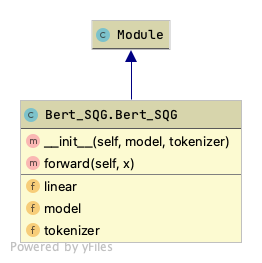
\includegraphics[scale=.45]{UML_diagrams/Bert_SQG.png}
				\caption{\texttt{BERT-SQG} Class\label{fig:bert_sqg}}
		\end{figure}
		\begin{figure}[h!]
			%\end{minipage}
			%\begin{minipage}[c]{0.45\textwidth}
				\centering
				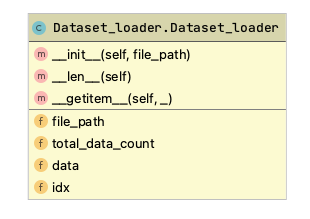
\includegraphics[scale=.5]{UML_diagrams/Dataset_loader.png}
				\caption{\texttt{Dataset\_loader} Class\label{fig:bert_dataset_loader}}
			%\end{minipage}
		\end{figure}
		
		\begin{figure}[h!]
			\centering
			\centering
			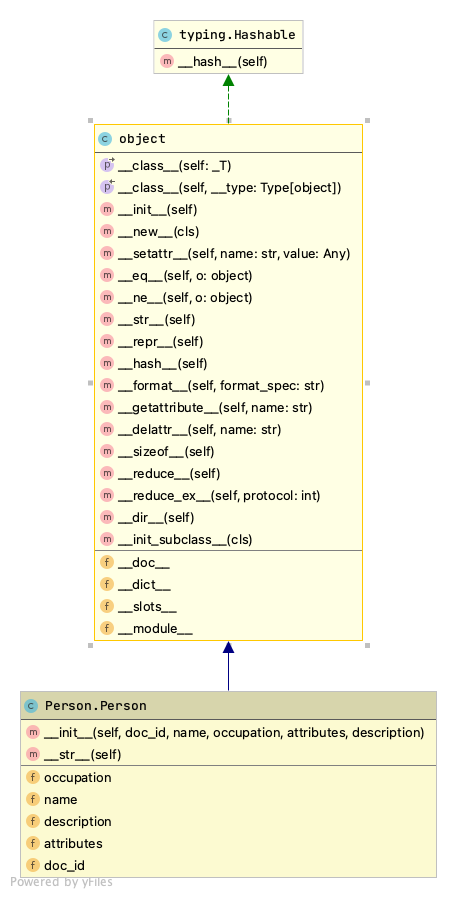
\includegraphics[scale=.5]{UML_diagrams/Person.png}
			\caption{\texttt{Person} Class\label{fig:dataset_person}}
		\end{figure}
		
		
		\begin{figure}[h!]
			\centering
			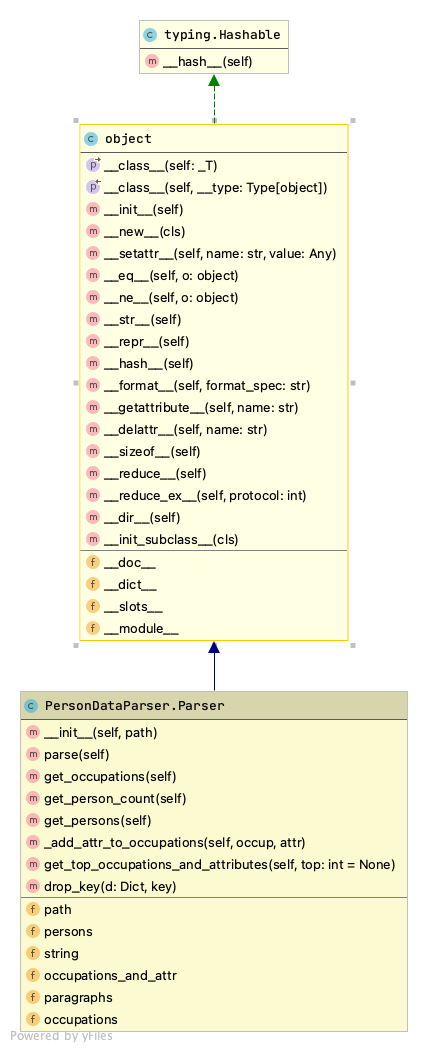
\includegraphics[scale=.55]{UML_diagrams/PersonDataParser.png}
			\caption{\texttt{PersonDataParser} Class\label{fig:dataset_persondataparser}}
		\end{figure}
		
	\end{appendix}
	
	
	\bibliographystyle{IEEEtranN}
	\bibliography{../bibliography/references}
\end{document}